\documentclass[12pt]{article}
\usepackage{amsmath, amssymb}
\usepackage{geometry}
\usepackage{tikz}
\usepackage{float}
\usetikzlibrary{arrows.meta, positioning}
\usepackage{graphicx}
\usepackage{booktabs}
\usepackage{hyperref}
\geometry{margin=1in}
\setlength{\parskip}{0.5em}
\setlength{\parindent}{1em}

\title{Modeling the Spread of Misinformation}
\author{Desiree DeGennaro}
\date{MATH 5131}

\begin{document}
\maketitle

\begin{abstract}
This paper builds a compartmental ODE model for how a false rumor spreads
through a population. The model
adapts three compartments: ignorants,
spreaders, and stiflers, and adds a debunking rate representing platform
intervention. The Jacobian produces two stable
policy thresholds: a minimum platform debunking rate $\delta^* = \beta N -
\alpha$ and a minimum pre-emptive awareness campaign coverage $p^* = 1 -
1/R_0$. A suggested time-delayed extension later incorporates a deliberation lag $\tau$
representing the time between exposure and the decision to share.
Simulations show that delay increases total
exposure even when the equilibrium remains stable. The output of the model
is three numbers that answer the question of how much intervention
is needed and in what form.
\end{abstract}

%------------------------------------------------------------------
\section{Introduction}
%------------------------------------------------------------------

Misinformation spreads fast and causes real damage before it dies out. The
World Health Organization has called the current information environment an
infodemic, where the volume of false and misleading content makes it hard
for accurate information to get through \cite{who2022}. Trafficking in people and recognition ability is
an example of where this becomes impactful. Many victims of human trafficking are
exploited by someone they know, are disproportionately people of color and
immigrants, and do not self-identify as trafficked. Starting in 2017, QAnon
ran a large-scale, global campaign built around a completely different story: elite
conspiracies, stranger kidnappings, and white children. By 2020, roughly 50
percent of Americans had seen QAnon content and about 14 percent identified
as believers \cite{prakash2022}. The result can be structural damage: survivors
whose experiences do not match the narrative stop coming forward, providers
get trained on the wrong profiles, real cases go unidentified.

This is a rumor spread problem and differential equations can model it.
Daley and Kendall (DK) introduced the compartmental rumor model in 1964 by
analogy with epidemic models \cite{daley1964}, and Piqueira et al. 
validated this framework specifically for fake news on social networks in 2020
\cite{piqueira2020}. This paper utilizes the approach to derive intervention thresholds from the stability analysis and connects all results directly to platform moderation and
community education strategies.

%------------------------------------------------------------------
\section{Part I: The ODE Model}
%------------------------------------------------------------------

\subsection{Compartments and Assumptions}

The population $N$ is fixed over the timescale of a viral event, which is
reasonable for a period of days to weeks. At any time $t \geq 0$, every
person is in one of three groups. $I(t)$ is ignorants: people who have not
heard the rumor. $S(t)$ is spreaders: people who have heard it and are
actively sharing it. $R(t)$ is stiflers: people who have heard it but
stopped sharing, either because they saw it debunked, lost interest, or
noticed that everyone around them already knew it. The conservation law
$$I(t) + S(t) + R(t) = N$$
holds for all $t \geq 0$. People only move $I \to S \to R$.

The difference between this model and a standard disease SIR model, infected people recover on their
own over time at a constant rate $\gamma$, giving a recovery term $-\gamma
I$. Here a spreader stops sharing specifically because they
contact someone who already knows the rumor, at which point it is no longer
worth sharing. The stifling rate therefore scales with contact between
spreaders and the already-informed population $S + R$, giving the term
$-\alpha S(S + R)$. Using $I + S + R = N$ this becomes $-\alpha S(N - I)$.
Stifling now is contact-driven, not time-driven, changing the
equilibrium structure.

The following assumptions are made:
\begin{enumerate}
    \item Population is homogeneously mixed: any person is equally likely to
    encounter any other person.
    \item When an ignorant contacts a spreader, the ignorant becomes a
    spreader at per-contact rate $\beta > 0$.
    \item When a spreader contacts any informed person, the spreader becomes
    a stifler at per-contact rate $\alpha > 0$.
    \item In the extended model, platforms remove false content at per-capita
    rate $\delta \geq 0$, converting spreaders to stiflers independently of
    contact.
\end{enumerate}

A compartment flow diagram is shown in Figure \ref{fig:compartments}.

\begin{figure}[h]
\centering
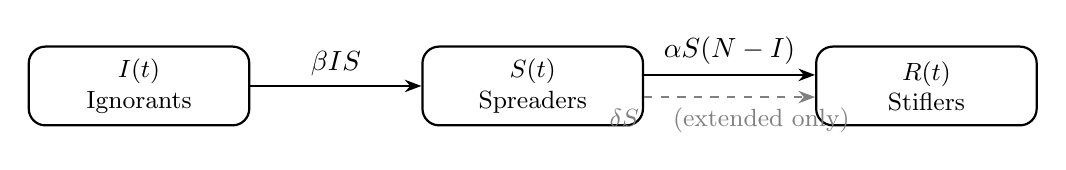
\begin{tikzpicture}[
  box/.style={draw, thick, rounded corners=6pt,
              minimum width=2.8cm, minimum height=1.0cm,
              align=center, font=\small},
  arr/.style={-{Stealth[length=6pt]}, thick},
  darr/.style={-{Stealth[length=6pt]}, thick, dashed, gray}
]
  \node[box] (I) at (0,0)   {$I(t)$\\Ignorants};
  \node[box] (S) at (5,0)   {$S(t)$\\Spreaders};
  \node[box] (R) at (10,0)  {$R(t)$\\Stiflers};
  \draw[arr] (I) -- (S)
    node[midway, above] {$\beta IS$};
  \draw[arr] ([yshift=4pt]S.east) -- ([yshift=4pt]R.west)
    node[midway, above] {$\alpha S(N-I)$};
  \draw[darr] ([yshift=-4pt]S.east) -- ([yshift=-4pt]R.west)
    node[midway, below] {\small $\delta S$ \quad (extended only)};
\end{tikzpicture}
\caption{Compartment flow diagram}
\label{fig:compartments}
\end{figure}

\subsection{The ODE Systems}

Each term below corresponds to one social interaction with a specific
per-contact rate. The term $\beta IS$ is contact between
ignorants and spreaders. The term $\alpha S(N - I)$ is contact
between spreaders and the informed population. The term $\delta S$ is
platform moderation acting independently of who talks to whom.

\textbf{Baseline model ($\delta = 0$):}
\begin{align*}
\dot{I} &= -\beta IS \\
\dot{S} &= \beta IS - \alpha S(N - I) \\
\dot{R} &= \alpha S(N - I)
\end{align*}

\textbf{Extended model ($\delta > 0$):}
\begin{align*}
\dot{I} &= -\beta IS \\
\dot{S} &= \beta IS - \alpha S(N - I) - \delta S \\
\dot{R} &= \alpha S(N - I) + \delta S
\end{align*}

Since $\dot{I} + \dot{S} + \dot{R} = 0$, the $\dot{R}$ equation is
redundant. All analysis reduces to the two-dimensional system in $I$ and
$S$ where $ I \geq 0,\; S \geq 0,\;
I + S \leq N\.$.

Parameters are defined:

\begin{table}[h]
\centering
\begin{tabular}{cll}
\toprule
Parameter & Description & Value Used \\
\midrule
$N$      & Fixed total population                     & 100 \\
$\beta$  & Per-contact spreading rate                 & 0.001 \\
$\alpha$ & Per-contact stifling rate                  & 0.01 \\
$\delta$ & Per-capita platform debunking rate         & 0.012 (extended) \\
\bottomrule
\end{tabular}
\caption{ODE model parameters. $\alpha > \beta$ means people lose interest
in sharing faster than they gain it, which is intentional and internally
consistent.}
\label{tab:ode_params}
\end{table}

\subsection{Equilibria}

Setting $\dot{I} = -\beta IS = 0$ gives $I = 0$ or $S = 0$. Setting
$\dot{S} = 0$ with $S = 0$ gives $0 = 0$, for any $I$. Setting
$I = 0$ in $\dot{S} = 0$ forces $S = 0$. Our equilibrium set is the
line
$$\mathcal{E} = \bigl\{(I^*,\, 0) : 0 \leq I^* \leq N\bigr\}.$$
Every equilibrium has $S = 0$: the rumor always dies out. What matters is
how much of the population is exposed before it does, which is $N - I^*$.

\subsection{The Reproduction Number}

$R_0$ is the expected number of new spreaders produced by one spreader
dropped into a fully ignorant population. One spreader at $t = 0$ with
$I(0) \approx N$ produces new spreaders at rate $\beta N$. The expected
time spent as a spreader before stifling is $1/\alpha$. So:
$$R_0 = \frac{\beta N}{\alpha} = \frac{0.001 \times 100}{0.01} = 10.$$
If $R_0 > 1$ the rumor spreads. If $R_0 < 1$ it dies immediately.

\subsection{The Critical Threshold $I_c$}

Setting $\dot{S} = 0$ with $S \neq 0$ in the spreader equation and solving
for $I$:
$$\beta I - \alpha(N - I) = 0 \implies (\alpha + \beta)I = \alpha N \implies
I_c = \frac{\alpha N}{\alpha + \beta} = \frac{(0.01)(100)}{0.011} = 90.9.$$
When $I > I_c$, $\dot{S} > 0$ and spreaders grow. When $I < I_c$, $\dot{S}
< 0$ and spreaders decline. Since $I(0) \approx N > I_c$, the rumor always
grows at first, peaks when $I(t)$ hits $I_c = 90.9$, then declines.

\subsection{Jacobian for Stability}

The Jacobian is from $F(I,S) = -\beta IS$ and
$G(I,S) = \beta IS - \alpha S(N-I)$:
$$J(I, S) =
\begin{pmatrix}
-\beta S & -\beta I \\
(\beta + \alpha)S & \beta I - \alpha(N-I) - \alpha S
\end{pmatrix}.$$
Because R=N - I - S is always determined by the other two variables, the third equation does not carry new information so the system reduces to two dimensions.
Then look at $(I^*, 0)$ by setting $S = 0$:
$$J^* =
\begin{pmatrix}
0 & -\beta I^* \\
0 & (\alpha + \beta)I^* - \alpha N
\end{pmatrix}.$$
The eigenvalues are:
$$\lambda_1 = 0, \qquad \lambda_2 = (\alpha + \beta)I^* - \alpha N.$$
$\lambda_1 = 0$ says there is a continuum of equilibria along
$S = 0$ not a single isolated fixed point. So stability is determinded by $\lambda_2$:
$$(\alpha + \beta)I^* < \alpha N \implies I^* < \frac{\alpha N}{\alpha +
\beta} = I_c.$$
So $\lambda_2 < 0$ when $I^* < I_c$ and the rumor dies, and $\lambda_2 > 0$
when $I^* > I_c$ and the rumor spreads. This is where $I_c = 90.9$ is validated. Piqueira et al. (2020) apply the identical Jacobian
approach to the DK fake-news model and validate the stability condition
\cite{piqueira2020}.

\subsection{Decision-Making Thresholds}

Next find the parameter value that pushes
$R_0$ below 1 for each intervention strategy.

\subsubsection{Minimum Platform Debunking Rate}

Adding $\delta$ changes the denominator of $R_0$:
$$R_0^\delta = \frac{\beta N}{\alpha + \delta}.$$
Setting $R_0^\delta < 1$ and solving for $\delta$:
$$\frac{\beta N}{\alpha + \delta} < 1 \implies \beta N < \alpha + \delta
\implies \delta > \beta N - \alpha.$$
\begin{equation*}
\boxed{\delta^* = \beta N - \alpha = (0.001)(100) - 0.01 = 0.09.}
\end{equation*}
$\beta N$ is the spreading pressure and $\alpha$ is the natural stifling
already in the system. Debunking only needs to close the gap between them.

\subsubsection{Minimum Awareness Campaign Coverage}

Pre-educating fraction $p$ of the population shrinks the effective ignorant
pool to $(1-p)N$:
$$R_0^{(p)} = \frac{\beta(1-p)N}{\alpha}.$$
Setting $R_0^{(p)} < 1$ and solving for $p$:
$$\frac{\beta(1-p)N}{\alpha} < 1 \implies 1 - p < \frac{\alpha}{\beta N}
\implies p > 1 - \frac{1}{R_0}.$$
\begin{equation*}
\boxed{p^* = 1 - \frac{1}{R_0} = 1 - \frac{1}{10} = 0.90.}
\end{equation*}
(As seen as the vaccination threshold in SIR.) For $R_0 = 10$,
reaching 90 percent of the community in advance prevents the rumor from
spreading at all.

%------------------------------------------------------------------
\section{Part II: The Time-Delayed Extension}
%------------------------------------------------------------------

\subsection{Motivation and Model}

The ODE model assumes that a person who hears a rumor immediately decides
whether to spread it or not. However, people may see
a post at any time and sit on it, then choose to share it hours or days later. To capture this,
a lag $\tau > 0$ is introduced, representing the time between
first exposure and the spreading decision.

From \cite{bf}, the delayed logistic model replaces
the instantaneous density term $X(t)/K$ with the lagged version
$X(t-\tau)/K$:
$$\frac{dX}{dt} = rX(t)\left(1 - \frac{X(t-\tau)}{K}\right).$$
But delayed feedback can cause
the system to overcompensate and this can produce oscillations when $\tau$ is large
relative to the response time $1/r$. Also, when people delay their sharing decision, the spreader inflow at time $t$
reflects contact information from time $t - \tau$, not from right now.
\begin{align*}
\dot{I}(t) &= -\beta I(t-\tau)\, S(t-\tau) \\
\dot{S}(t) &= \beta I(t-\tau)\, S(t-\tau) - \alpha S(t)(N - I(t)) \\
\dot{R}(t) &= \alpha S(t)(N - I(t))
\end{align*}

The stifling term $\alpha S(t)(N - I(t))$ stays undelayed because going
quiet is an immediate response: a spreader encounters someone who already
knows the rumor and stops in that moment. Only the spreading decision is
lagged.  The
new parameter introduced is simulated at time units 0, 10, 30.
\subsection{Stability of the Delayed System}
Next, test what happens when
spreaders are given a small nudge away from zero by assuming $S(t) = e^{\lambda t}$ and plug it in. If
$\lambda < 0$ the spreaders decay back to zero and the equilibrium is stable; if $\lambda > 0$ they grow and it is unstable. The complication is that the delay term $S(t - \tau)$ becomes
$e^{\lambda t} e^{-\lambda\tau}$ after substitution, meaning $\lambda$ now
appears in the equation in two places so theres no clean formula for $\lambda$ \cite{bf}.

The simulation runs the delayed model forward from a small perturbation and check whether $S(t)$ decays or grows.
Then the boundary between stable and unstable by setting
$\lambda = i\omega$ is the point where the
system tips from decaying to oscillating. Solving the resulting real and
imaginary parts finds the critical delay $\tau^*$ where
stability changes, if there is one. For small-$\tau$ approximation
for small delays, $e^{-\lambda\tau} \approx 1 - \lambda\tau$, gets:
$$\lambda \approx \frac{(\alpha+\beta)I^* - \alpha N}{1 + \beta I^* \tau}.$$
The numerator is $\lambda_2$ from the Jacobian originally. When $I^* < I_c = 90.9$, the numerator is negative, so
$\lambda < 0$ for any small $\tau$ as well. Small delays dont change the
stability from the original system. When $I^* < I_c = 90.9$ that numerator is
negative, so $\lambda < 0$ for any $\tau > 0$ as well. This means small
delays do not destabilize the rumor-free equilibrium. The ODE stability carries over for small $\tau$, and the threshold
$I_c = 90.9$ still decides whether spreaders grow or decay.

%------------------------------------------------------------------
\section{Simulations}
%------------------------------------------------------------------
All simulations are implemented in Python using \texttt{numpy}, 
\texttt{scipy.integrate.solve\_ivp} for the ODE systems, 
\texttt{scipy.optimize.fsolve} for root-finding on the characteristic 
equation, and \texttt{matplotlib} for all plots. The delayed model is solved using 
a forward Euler strategy with history tracking, where lagged values 
$I(t-\tau)$ and $S(t-\tau)$ are looked up from stored arrays at each time 
step, mirroring the approach in Barnes and Fulford 
\cite{bf}.

Using $\beta = 0.001$, $\alpha = 0.01$, $N = 100$,
$I(0) = 99$, $S(0) = 1$, $R(0) = 0$. Derived $R_0 = 10$,
$I_c = 90.9$, $\delta^* = 0.09$, $p^* = 0.90$.


\begin{figure}[H]
    \centering
    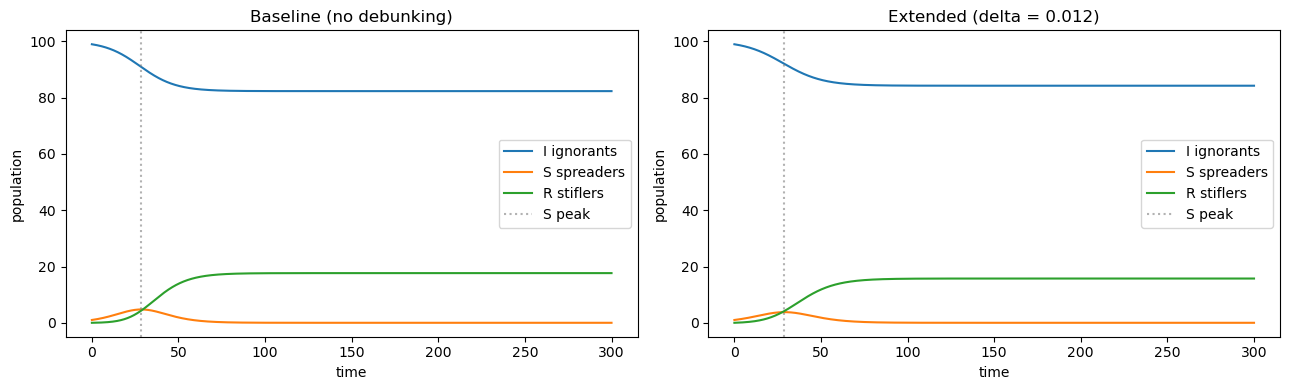
\includegraphics[width=1\linewidth]{image2.png}
\end{figure}
\textbf{Figure 2: Time series.} Without intervention, $I(t)$ falls from 99
to about 83, meaning 17 percent of the population is exposed. $S(t)$
peaks around $t = 30$ when $I$ crosses the critical threshold
$I_c = 90.9$ from the nullcline again. With $\delta = 0.012$,
which is below the minimum debunking rate $\delta^* = 0.09$, exposure drops to 15 percent. Less than threshold debunking still helps.

\begin{figure}[H]
    \centering
    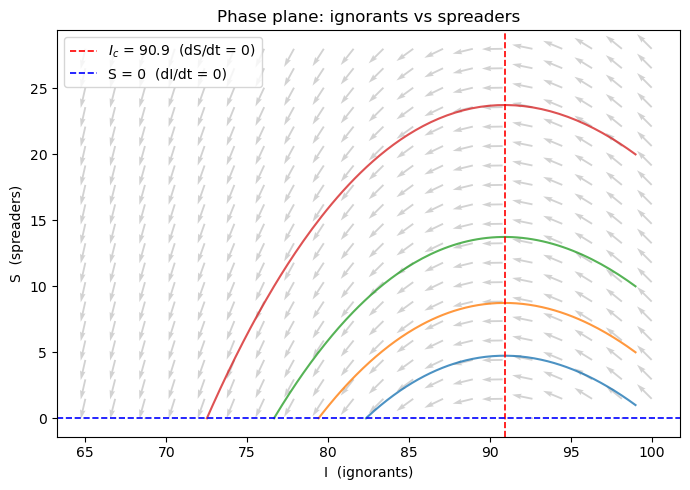
\includegraphics[width=.5\linewidth]{image3.png}
\end{figure}

\textbf{Figure 3: Phase plane.} Trajectories are shown with $I(0) = 99$
and $S(0) \in \{1, 5, 10, 20\}$. Since $\dot{I} = -\beta IS < 0$ always everything moves and vector field point left, peaks at
the nullcline $I = I_c = 90.9$ and falls to $S = 0$. The vector field is the visual version of the eigenvalue result $\lambda_2 > 0$
on the right, $\lambda_2 < 0$ on the left.






\begin{figure}[H]
    \centering
    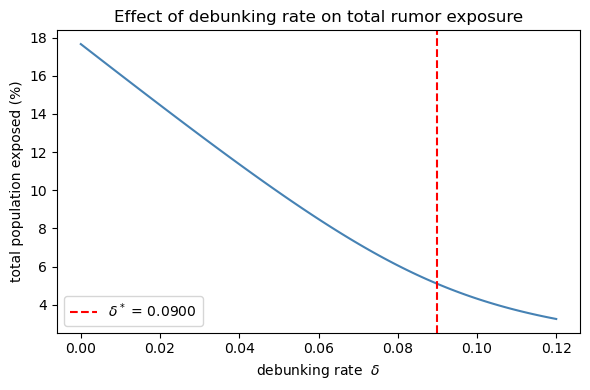
\includegraphics[width=0.5\linewidth]{5.png}
\end{figure}
\textbf{Figure 4: Decision boundary.} At $\delta = 0$, 17.5 percent
of the population is exposed. At the minimum debunking rate $\delta^* =
0.09$, exposure drops to about 4 percent. The curve is steep early, so the
first increments of moderation do the most work. Reaching $\delta^*$ is not
required to meaningfully reduce harm.




\begin{figure}[H]
    \centering
    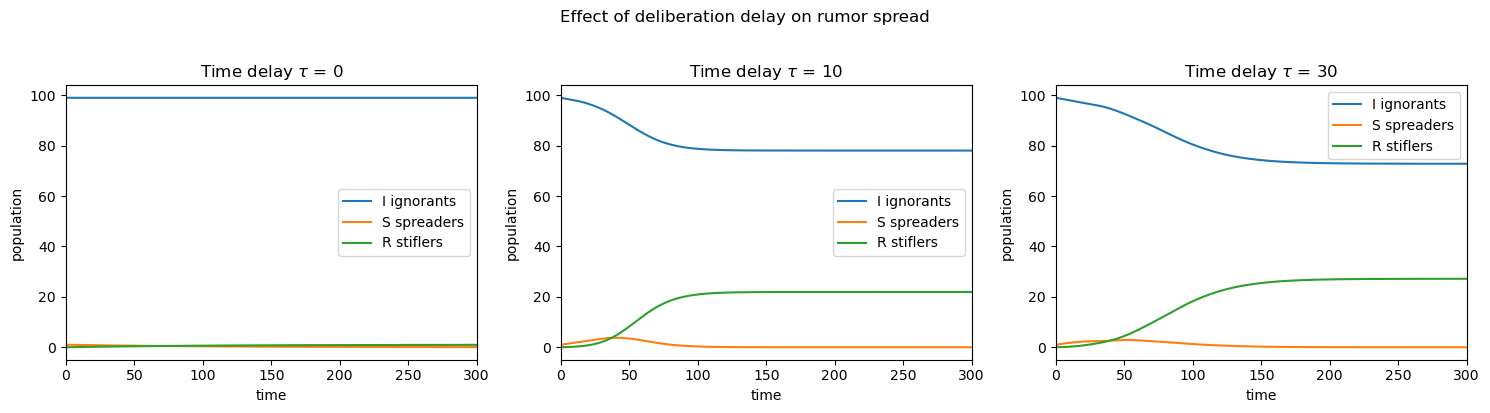
\includegraphics[width=1\linewidth]{7.png}
\end{figure}

\textbf{Figure 5: Time-delay simulations.} In Python an Euler scheme with history tracking \cite{bf} proposes results for $\tau = 0$, $\tau = 10$, and $\tau = 30$.

The most immediate finding and difference is that delay increases total exposure: at
$\tau = 0$, 1 percent of the population is reached; at
$\tau = 10$, this rises to 21.9 percent; at $\tau = 30$, it reaches 27.2
percent. This is counterintuitive. A person deliberating longer before
sharing does not reduce harm, it increases it. The reason is that the
delayed spreading term $\beta I(t-\tau)S(t-\tau)$ feeds new spreaders based
on stale contact information. The system loses real-time awareness of how
much spreading pressure exists, so spreaders accumulate more slowly but
persist longer before stifling catches up.

Solving for the roots found no imaginary
axis crossing so
the equilibrium stays stable for all $\tau$. The rumor still
burns out, just more slowly and with more total damage. Platforms that rely
on organic stifling to kill a rumor cannot count on it acting quickly when
users deliberate before sharing. Since stifling is instantaneous but new
spreaders arrive late, the natural self-regulation weakens as $\tau$ grows.
This makes active platform debunking at $\delta > \delta^* = 0.09$ more
important, not less, in a world where deliberation delays are realistic.

%------------------------------------------------------------------
\section{Conclusions}
%------------------------------------------------------------------

Our model pushes platforms to need $\delta > 0.09$ to suppress
a rumor from the start. Awareness organizations need to reach at least 90
percent of the target community before the rumor enters to prevent it from
spreading at all. When people delay before sharing, total exposure
increases from 1 percent at $\tau = 0$ to 27 percent at $\tau = 30$,
so the natural self-regulation of the rumor weakens as the deliberation time to share
window grows. Even below both thresholds though, moderation reduces total
exposure.

For the trafficking context, these results support two concrete strategies.
Platforms should maintain content moderation above $\delta^* = 0.09$ for
known false trafficking narratives, the time-delay result making this
more urgent.
Platform-level intervention that acts in real time becomes the more reliable
lever. Anti-trafficking organizations should treat pre-emptive community
education as the proactive complement: reaching 90 percent of a community
with accurate information about what trafficking actually looks like prevents the QAnon-style narrative from taking hold before
it enters. This is consistent with the recommendations in Prakash et al. who call for health sector education to reach diverse demographics
before disinformation saturates the space \cite{prakash2022}.

The main limitation is the homogeneous mixing assumption. Real social media
has echo chambers where spreaders rarely encounter informed people, keeping
the stifling term $\alpha S(N - I)$ small and letting the rumor persist
longer than this model predicts. The time-delay extension compounds this:
in a clustered network with delayed sharing behavior, both $\delta^* = 0.09$
and $p^* = 0.90$ would be higher than the values derived here. A network
model where $N$ is replaced by a local cluster/echo chamber size and $\tau$ is
estimated from platform engagement data is a future step for making
these thresholds more realistic.

%------------------------------------------------------------------
\begin{thebibliography}{9}

\bibitem{daley1964}
D.~J. Daley and D.~G. Kendall,
``Epidemics and Rumours,''
\textit{Nature}, vol.~204, p.~1118, 1964.

\bibitem{bf}
B.~Barnes and G.~Fulford,
\textit{Mathematical Modeling with Case Studies}, 3rd ed.
CRC Press, 2015.

\bibitem{prakash2022}
J.~Prakash, T.~B. Erickson, and H.~Stoklosa,
``Human Trafficking and the Growing Malady of Disinformation,''
\textit{Frontiers in Public Health}, vol.~10, 987159, 2022.

\bibitem{piqueira2020}
J.~R.~C. Piqueira, M.~Zilbovicius, and C.~M. Batistela,
``Daley-Kendal Models in Fake-News Scenario,''
\textit{Physica A}, vol.~548, 123406, 2020.

\bibitem{who2022}
World Health Organization,
``Infodemic,'' 2022.
Available at: \url{https://www.who.int/health-topics/infodemic}

\end{thebibliography}

\end{document}